\documentclass[book.tex]{subfiles}
\begin{document}
\section{Source Code}

Includel list of all files.\\
Include cloc stats.

 \begin{fancyquotes}
   We didn't have spell checkers in our editors back then, and I always had poor spelling.  The word “collumn” appears in the source code dozens of times.  After I released the source code, one of the emails that stands out in memory read:
 \bigskip \\
It's "COLUMN", you dumb @\#\$\% !\\
 \bigskip \\
\textbf{John Carmack - Programmer}
 \end{fancyquotes}



\section{Architecture}


\begin{figure}[H]
  \centering
 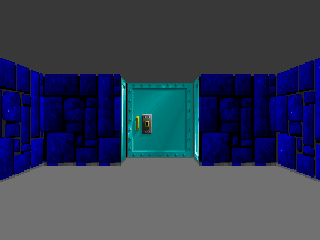
\includegraphics[scale=1.3]{imgs/ray_caster_explained/beginning.png}
 \caption{Raycasting 1: Screenshot} \label{fig:Raycasting2Drawing}
\end{figure}

\begin{figure}[H]
  \centering
  \documentclass[crop,tikz]{standalone}% 'crop' is the default for v1.0, before it was 'preview'
%\usetikzlibrary{...}% tikz package already loaded by 'tikz' option
\begin{document}

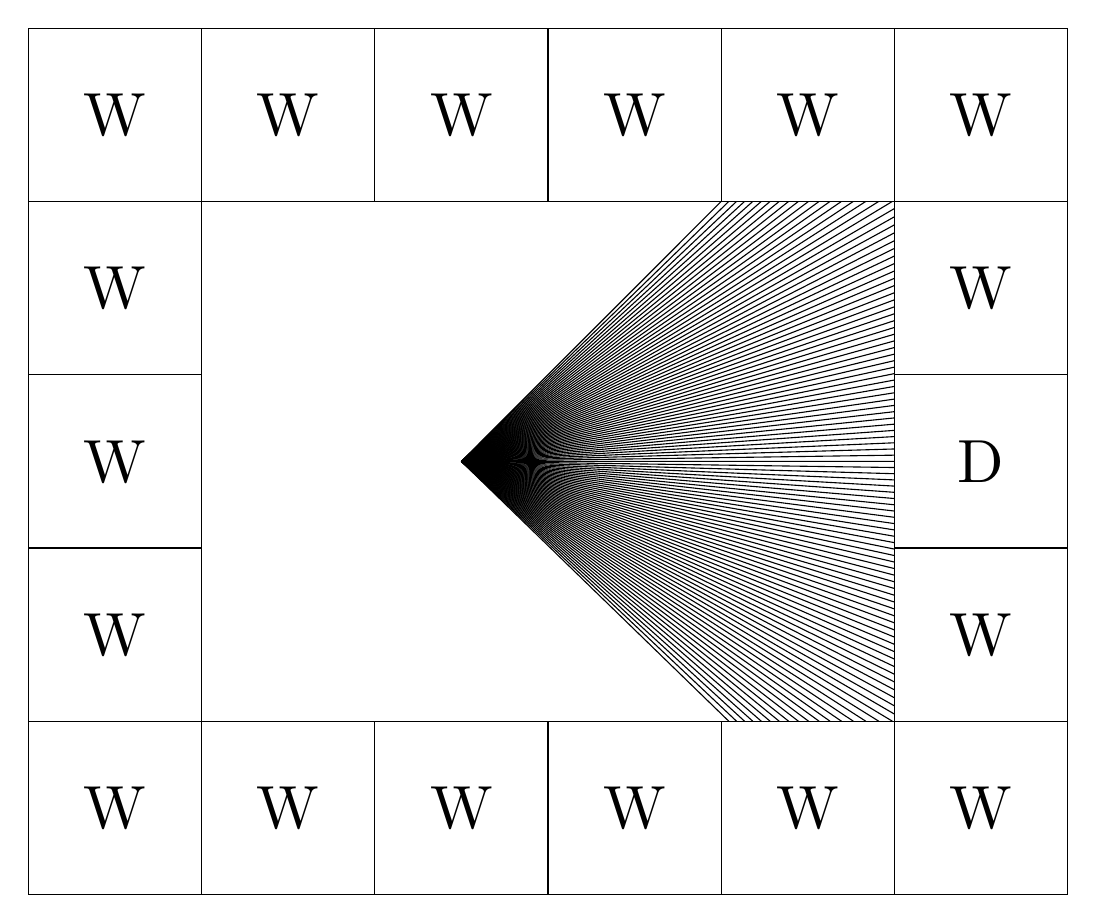
\begin{tikzpicture}[y=-1cm,scale=2.2, every node/.style={scale=2.2}]


\draw (27,55) rectangle (28,56) node[pos=.5] {W};
\draw (27,56) rectangle (28,57) node[pos=.5] {W};
\draw (27,57) rectangle (28,58) node[pos=.5] {W};
\draw (27,58) rectangle (28,59) node[pos=.5] {W};
\draw (27,59) rectangle (28,60) node[pos=.5] {W};
\draw (28,55) rectangle (29,56) node[pos=.5] {W};
\draw (28,59) rectangle (29,60) node[pos=.5] {W};
\draw (29,55) rectangle (30,56) node[pos=.5] {W};
\draw (29,59) rectangle (30,60) node[pos=.5] {W};
\draw (30,55) rectangle (31,56) node[pos=.5] {W};
\draw (30,59) rectangle (31,60) node[pos=.5] {W};
\draw (31,55) rectangle (32,56) node[pos=.5] {W};
\draw (31,59) rectangle (32,60) node[pos=.5] {W};
\draw (32,55) rectangle (33,56) node[pos=.5] {W};
\draw (32,56) rectangle (33,57) node[pos=.5] {W};
\draw (32,57) rectangle (33,58) node[pos=.5] {D};
\draw (32,58) rectangle (33,59) node[pos=.5] {W};
\draw (32,59) rectangle (33,60) node[pos=.5] {W};
\draw[thin,black] (29.500000,57.500000) -- (30.999512,56.000000);
\draw[thin,black] (29.500000,57.500000) -- (31.042963,56.000000);
\draw[thin,black] (29.500000,57.500000) -- (31.087708,56.000000);
\draw[thin,black] (29.500000,57.500000) -- (31.133820,56.000000);
\draw[thin,black] (29.500000,57.500000) -- (31.181396,56.000000);
\draw[thin,black] (29.500000,57.500000) -- (31.230524,56.000000);
\draw[thin,black] (29.500000,57.500000) -- (31.281282,56.000000);
\draw[thin,black] (29.500000,57.500000) -- (31.333809,56.000000);
\draw[thin,black] (29.500000,57.500000) -- (31.388191,56.000000);
\draw[thin,black] (29.500000,57.500000) -- (31.444569,56.000000);
\draw[thin,black] (29.500000,57.500000) -- (31.503065,56.000000);
\draw[thin,black] (29.500000,57.500000) -- (31.563847,56.000000);
\draw[thin,black] (29.500000,57.500000) -- (31.627069,56.000000);
\draw[thin,black] (29.500000,57.500000) -- (31.692896,56.000000);
\draw[thin,black] (29.500000,57.500000) -- (31.761520,56.000000);
\draw[thin,black] (29.500000,57.500000) -- (31.833183,56.000000);
\draw[thin,black] (29.500000,57.500000) -- (31.908092,56.000000);
\draw[thin,black] (29.500000,57.500000) -- (31.986519,56.000000);
\draw[thin,black] (29.500000,57.500000) -- (32.000000,56.040142);
\draw[thin,black] (29.500000,57.500000) -- (32.000000,56.087624);
\draw[thin,black] (29.500000,57.500000) -- (32.000000,56.134342);
\draw[thin,black] (29.500000,57.500000) -- (32.000000,56.180344);
\draw[thin,black] (29.500000,57.500000) -- (32.000000,56.225647);
\draw[thin,black] (29.500000,57.500000) -- (32.000000,56.270302);
\draw[thin,black] (29.500000,57.500000) -- (32.000000,56.314327);
\draw[thin,black] (29.500000,57.500000) -- (32.000000,56.357765);
\draw[thin,black] (29.500000,57.500000) -- (32.000000,56.400642);
\draw[thin,black] (29.500000,57.500000) -- (32.000000,56.442978);
\draw[thin,black] (29.500000,57.500000) -- (32.000000,56.484814);
\draw[thin,black] (29.500000,57.500000) -- (32.000000,56.526161);
\draw[thin,black] (29.500000,57.500000) -- (32.000000,56.567047);
\draw[thin,black] (29.500000,57.500000) -- (32.000000,56.607506);
\draw[thin,black] (29.500000,57.500000) -- (32.000000,56.647556);
\draw[thin,black] (29.500000,57.500000) -- (32.000000,56.687210);
\draw[thin,black] (29.500000,57.500000) -- (32.000000,56.726501);
\draw[thin,black] (29.500000,57.500000) -- (32.000000,56.765450);
\draw[thin,black] (29.500000,57.500000) -- (32.000000,56.804073);
\draw[thin,black] (29.500000,57.500000) -- (32.000000,56.842388);
\draw[thin,black] (29.500000,57.500000) -- (32.000000,56.880417);
\draw[thin,black] (29.500000,57.500000) -- (32.000000,56.918182);
\draw[thin,black] (29.500000,57.500000) -- (32.000000,56.955688);
\draw[thin,black] (29.500000,57.500000) -- (32.000000,56.992966);
\draw[thin,black] (29.500000,57.500000) -- (32.000000,57.030029);
\draw[thin,black] (29.500000,57.500000) -- (32.000000,57.066895);
\draw[thin,black] (29.500000,57.500000) -- (32.000000,57.103577);
\draw[thin,black] (29.500000,57.500000) -- (32.000000,57.140095);
\draw[thin,black] (29.500000,57.500000) -- (32.000000,57.176460);
\draw[thin,black] (29.500000,57.500000) -- (32.000000,57.212692);
\draw[thin,black] (29.500000,57.500000) -- (32.000000,57.248806);
\draw[thin,black] (29.500000,57.500000) -- (32.000000,57.284813);
\draw[thin,black] (29.500000,57.500000) -- (32.000000,57.320736);
\draw[thin,black] (29.500000,57.500000) -- (32.000000,57.356586);
\draw[thin,black] (29.500000,57.500000) -- (32.000000,57.392376);
\draw[thin,black] (29.500000,57.500000) -- (32.000000,57.428120);
\draw[thin,black] (29.500000,57.500000) -- (32.000000,57.463837);
\draw[thin,black] (29.500000,57.500000) -- (32.000000,57.499535);
\draw[thin,black] (29.500000,57.500000) -- (32.000000,57.535236);
\draw[thin,black] (29.500000,57.500000) -- (32.000000,57.570950);
\draw[thin,black] (29.500000,57.500000) -- (32.000000,57.606701);
\draw[thin,black] (29.500000,57.500000) -- (32.000000,57.642487);
\draw[thin,black] (29.500000,57.500000) -- (32.000000,57.678333);
\draw[thin,black] (29.500000,57.500000) -- (32.000000,57.714252);
\draw[thin,black] (29.500000,57.500000) -- (32.000000,57.750259);
\draw[thin,black] (29.500000,57.500000) -- (32.000000,57.786369);
\draw[thin,black] (29.500000,57.500000) -- (32.000000,57.822598);
\draw[thin,black] (29.500000,57.500000) -- (32.000000,57.858963);
\draw[thin,black] (29.500000,57.500000) -- (32.000000,57.895473);
\draw[thin,black] (29.500000,57.500000) -- (32.000000,57.932152);
\draw[thin,black] (29.500000,57.500000) -- (32.000000,57.969009);
\draw[thin,black] (29.500000,57.500000) -- (32.000000,58.006065);
\draw[thin,black] (29.500000,57.500000) -- (32.000000,58.043343);
\draw[thin,black] (29.500000,57.500000) -- (32.000000,58.080845);
\draw[thin,black] (29.500000,57.500000) -- (32.000000,58.118599);
\draw[thin,black] (29.500000,57.500000) -- (32.000000,58.156616);
\draw[thin,black] (29.500000,57.500000) -- (32.000000,58.194931);
\draw[thin,black] (29.500000,57.500000) -- (32.000000,58.233540);
\draw[thin,black] (29.500000,57.500000) -- (32.000000,58.272480);
\draw[thin,black] (29.500000,57.500000) -- (32.000000,58.311760);
\draw[thin,black] (29.500000,57.500000) -- (32.000000,58.351410);
\draw[thin,black] (29.500000,57.500000) -- (32.000000,58.391445);
\draw[thin,black] (29.500000,57.500000) -- (32.000000,58.431892);
\draw[thin,black] (29.500000,57.500000) -- (32.000000,58.472771);
\draw[thin,black] (29.500000,57.500000) -- (32.000000,58.514107);
\draw[thin,black] (29.500000,57.500000) -- (32.000000,58.555927);
\draw[thin,black] (29.500000,57.500000) -- (32.000000,58.598251);
\draw[thin,black] (29.500000,57.500000) -- (32.000000,58.641113);
\draw[thin,black] (29.500000,57.500000) -- (32.000000,58.684536);
\draw[thin,black] (29.500000,57.500000) -- (32.000000,58.728550);
\draw[thin,black] (29.500000,57.500000) -- (32.000000,58.773186);
\draw[thin,black] (29.500000,57.500000) -- (32.000000,58.818478);
\draw[thin,black] (29.500000,57.500000) -- (32.000000,58.864452);
\draw[thin,black] (29.500000,57.500000) -- (32.000000,58.911156);
\draw[thin,black] (29.500000,57.500000) -- (32.000000,58.958611);
\draw[thin,black] (29.500000,57.500000) -- (31.988605,59.000000);
\draw[thin,black] (29.500000,57.500000) -- (31.910082,59.000000);
\draw[thin,black] (29.500000,57.500000) -- (31.835087,59.000000);
\draw[thin,black] (29.500000,57.500000) -- (31.763346,59.000000);
\draw[thin,black] (29.500000,57.500000) -- (31.694633,59.000000);
\draw[thin,black] (29.500000,57.500000) -- (31.628738,59.000000);
\draw[thin,black] (29.500000,57.500000) -- (31.565458,59.000000);
\draw[thin,black] (29.500000,57.500000) -- (31.504620,59.000000);
\draw[thin,black] (29.500000,57.500000) -- (31.446058,59.000000);
\draw[thin,black] (29.500000,57.500000) -- (31.389629,59.000000);
\draw[thin,black] (29.500000,57.500000) -- (31.335192,59.000000);
\draw[thin,black] (29.500000,57.500000) -- (31.282625,59.000000);
\draw[thin,black] (29.500000,57.500000) -- (31.231813,59.000000);
\draw[thin,black] (29.500000,57.500000) -- (31.182652,59.000000);
\draw[thin,black] (29.500000,57.500000) -- (31.135036,59.000000);
\draw[thin,black] (29.500000,57.500000) -- (31.088884,59.000000);
\draw[thin,black] (29.500000,57.500000) -- (31.044106,59.000000);
\end{tikzpicture}
\end{document}
 \caption{Raycasting 1: Drawing} \label{fig:Raycasting1}
\end{figure}




\begin{figure}[H]
  \centering
 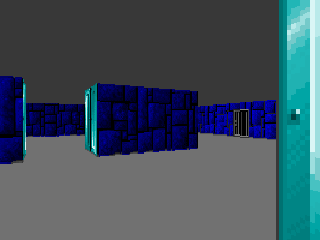
\includegraphics[scale=1.3]{imgs/ray_caster_explained/out_door.png}
 \caption{Raycasting 2: Screenshot} \label{fig:Raycasting2Drawing}
\end{figure}

\begin{figure}[H]
\centering
 
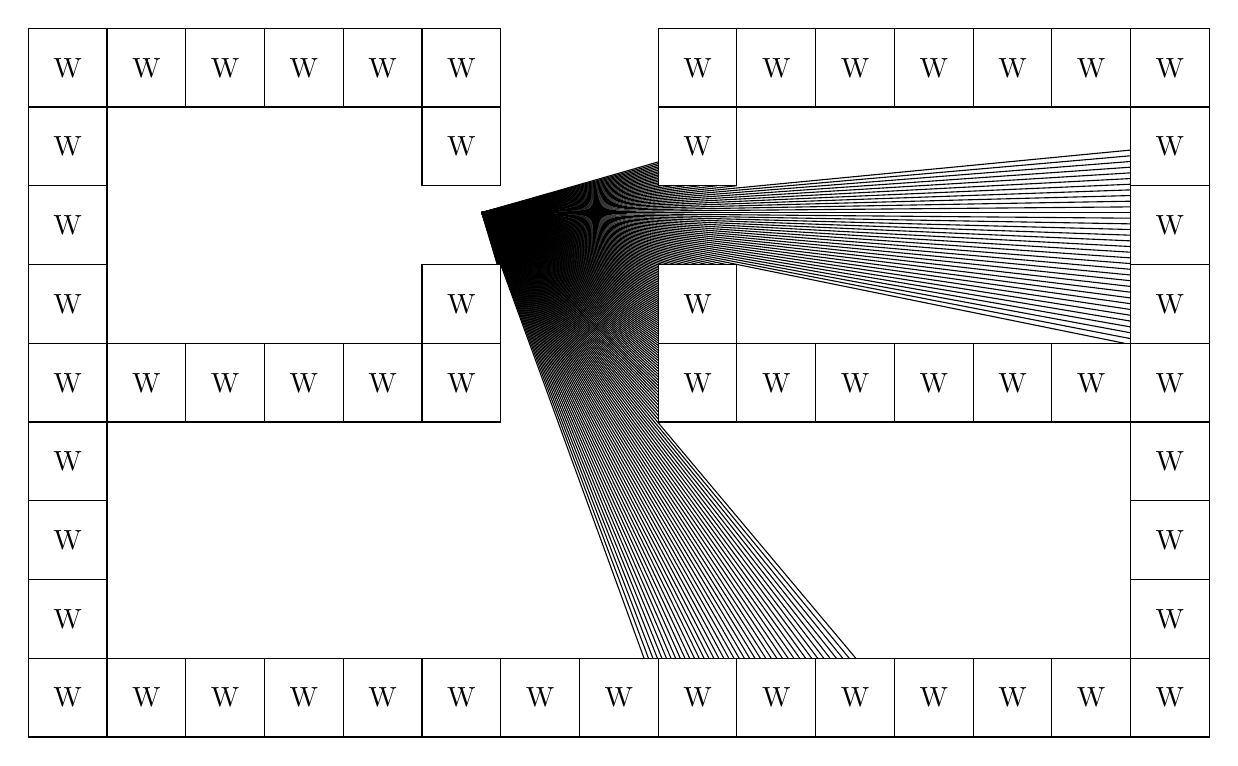
\begin{tikzpicture}[y=-1cm,scale=1.0, every node/.style={scale=1.0}]


\draw (27,55) rectangle (28,56) node[pos=.5] {W};
\draw (27,56) rectangle (28,57) node[pos=.5] {W};
\draw (27,57) rectangle (28,58) node[pos=.5] {W};
\draw (27,58) rectangle (28,59) node[pos=.5] {W};
\draw (27,59) rectangle (28,60) node[pos=.5] {W};
\draw (27,60) rectangle (28,61) node[pos=.5] {W};
\draw (27,61) rectangle (28,62) node[pos=.5] {W};
\draw (27,62) rectangle (28,63) node[pos=.5] {W};
\draw (27,63) rectangle (28,64) node[pos=.5] {W};
\draw (28,55) rectangle (29,56) node[pos=.5] {W};
\draw (28,59) rectangle (29,60) node[pos=.5] {W};
\draw (28,63) rectangle (29,64) node[pos=.5] {W};
\draw (29,55) rectangle (30,56) node[pos=.5] {W};
\draw (29,59) rectangle (30,60) node[pos=.5] {W};
\draw (29,63) rectangle (30,64) node[pos=.5] {W};
\draw (30,55) rectangle (31,56) node[pos=.5] {W};
\draw (30,59) rectangle (31,60) node[pos=.5] {W};
\draw (30,63) rectangle (31,64) node[pos=.5] {W};
\draw (31,55) rectangle (32,56) node[pos=.5] {W};
\draw (31,59) rectangle (32,60) node[pos=.5] {W};
\draw (31,63) rectangle (32,64) node[pos=.5] {W};
\draw (32,55) rectangle (33,56) node[pos=.5] {W};
\draw (32,56) rectangle (33,57) node[pos=.5] {W};
\draw (32,58) rectangle (33,59) node[pos=.5] {W};
\draw (32,59) rectangle (33,60) node[pos=.5] {W};
\draw (32,63) rectangle (33,64) node[pos=.5] {W};
\draw (33,63) rectangle (34,64) node[pos=.5] {W};
\draw (34,63) rectangle (35,64) node[pos=.5] {W};
\draw (35,55) rectangle (36,56) node[pos=.5] {W};
\draw (35,56) rectangle (36,57) node[pos=.5] {W};
\draw (35,58) rectangle (36,59) node[pos=.5] {W};
\draw (35,59) rectangle (36,60) node[pos=.5] {W};
\draw (35,63) rectangle (36,64) node[pos=.5] {W};
\draw (36,55) rectangle (37,56) node[pos=.5] {W};
\draw (36,59) rectangle (37,60) node[pos=.5] {W};
\draw (36,63) rectangle (37,64) node[pos=.5] {W};
\draw (37,55) rectangle (38,56) node[pos=.5] {W};
\draw (37,59) rectangle (38,60) node[pos=.5] {W};
\draw (37,63) rectangle (38,64) node[pos=.5] {W};
\draw (38,55) rectangle (39,56) node[pos=.5] {W};
\draw (38,59) rectangle (39,60) node[pos=.5] {W};
\draw (38,63) rectangle (39,64) node[pos=.5] {W};
\draw (39,55) rectangle (40,56) node[pos=.5] {W};
\draw (39,59) rectangle (40,60) node[pos=.5] {W};
\draw (39,63) rectangle (40,64) node[pos=.5] {W};
\draw (40,55) rectangle (41,56) node[pos=.5] {W};
\draw (40,59) rectangle (41,60) node[pos=.5] {W};
\draw (40,63) rectangle (41,64) node[pos=.5] {W};
\draw (41,55) rectangle (42,56) node[pos=.5] {W};
\draw (41,56) rectangle (42,57) node[pos=.5] {W};
\draw (41,57) rectangle (42,58) node[pos=.5] {W};
\draw (41,58) rectangle (42,59) node[pos=.5] {W};
\draw (41,59) rectangle (42,60) node[pos=.5] {W};
\draw (41,60) rectangle (42,61) node[pos=.5] {W};
\draw (41,61) rectangle (42,62) node[pos=.5] {W};
\draw (41,62) rectangle (42,63) node[pos=.5] {W};
\draw (41,63) rectangle (42,64) node[pos=.5] {W};
\draw[thin,black] (32.759998,57.340000) -- (35.000000,56.697712);
\draw[thin,black] (32.759998,57.340000) -- (35.000000,56.718815);
\draw[thin,black] (32.759998,57.340000) -- (35.000000,56.739815);
\draw[thin,black] (32.759998,57.340000) -- (35.000000,56.760712);
\draw[thin,black] (32.759998,57.340000) -- (35.000000,56.781525);
\draw[thin,black] (32.759998,57.340000) -- (35.000000,56.802242);
\draw[thin,black] (32.759998,57.340000) -- (35.000000,56.822868);
\draw[thin,black] (32.759998,57.340000) -- (35.000000,56.843414);
\draw[thin,black] (32.759998,57.340000) -- (35.000000,56.863884);
\draw[thin,black] (32.759998,57.340000) -- (35.000000,56.884285);
\draw[thin,black] (32.759998,57.340000) -- (35.000000,56.904602);
\draw[thin,black] (32.759998,57.340000) -- (35.000000,56.924854);
\draw[thin,black] (32.759998,57.340000) -- (35.000000,56.945038);
\draw[thin,black] (32.759998,57.340000) -- (35.000000,56.965164);
\draw[thin,black] (32.759998,57.340000) -- (35.000000,56.985229);
\draw[thin,black] (32.759998,57.340000) -- (35.035076,57.000000);
\draw[thin,black] (32.759998,57.340000) -- (35.179306,57.000000);
\draw[thin,black] (32.759998,57.340000) -- (35.342648,57.000000);
\draw[thin,black] (32.759998,57.340000) -- (35.529148,57.000000);
\draw[thin,black] (32.759998,57.340000) -- (35.744217,57.000000);
\draw[thin,black] (32.759998,57.340000) -- (35.994972,57.000000);
\draw[thin,black] (32.759998,57.340000) -- (41.000000,56.546600);
\draw[thin,black] (32.759998,57.340000) -- (41.000000,56.619114);
\draw[thin,black] (32.759998,57.340000) -- (41.000000,56.691517);
\draw[thin,black] (32.759998,57.340000) -- (41.000000,56.763821);
\draw[thin,black] (32.759998,57.340000) -- (41.000000,56.836033);
\draw[thin,black] (32.759998,57.340000) -- (41.000000,56.908173);
\draw[thin,black] (32.759998,57.340000) -- (41.000000,56.980244);
\draw[thin,black] (32.759998,57.340000) -- (41.000000,57.052261);
\draw[thin,black] (32.759998,57.340000) -- (41.000000,57.124237);
\draw[thin,black] (32.759998,57.340000) -- (41.000000,57.196175);
\draw[thin,black] (32.759998,57.340000) -- (41.000000,57.268093);
\draw[thin,black] (32.759998,57.340000) -- (41.000000,57.340000);
\draw[thin,black] (32.759998,57.340000) -- (41.000000,57.411907);
\draw[thin,black] (32.759998,57.340000) -- (41.000000,57.483826);
\draw[thin,black] (32.759998,57.340000) -- (41.000000,57.555763);
\draw[thin,black] (32.759998,57.340000) -- (41.000000,57.627739);
\draw[thin,black] (32.759998,57.340000) -- (41.000000,57.699757);
\draw[thin,black] (32.759998,57.340000) -- (41.000000,57.771828);
\draw[thin,black] (32.759998,57.340000) -- (41.000000,57.843967);
\draw[thin,black] (32.759998,57.340000) -- (41.000000,57.916180);
\draw[thin,black] (32.759998,57.340000) -- (41.000000,57.988483);
\draw[thin,black] (32.759998,57.340000) -- (41.000000,58.060886);
\draw[thin,black] (32.759998,57.340000) -- (41.000000,58.133400);
\draw[thin,black] (32.759998,57.340000) -- (41.000000,58.206036);
\draw[thin,black] (32.759998,57.340000) -- (41.000000,58.278805);
\draw[thin,black] (32.759998,57.340000) -- (41.000000,58.351715);
\draw[thin,black] (32.759998,57.340000) -- (41.000000,58.424782);
\draw[thin,black] (32.759998,57.340000) -- (41.000000,58.498020);
\draw[thin,black] (32.759998,57.340000) -- (41.000000,58.571438);
\draw[thin,black] (32.759998,57.340000) -- (41.000000,58.645050);
\draw[thin,black] (32.759998,57.340000) -- (41.000000,58.718861);
\draw[thin,black] (32.759998,57.340000) -- (41.000000,58.792892);
\draw[thin,black] (32.759998,57.340000) -- (41.000000,58.867146);
\draw[thin,black] (32.759998,57.340000) -- (41.000000,58.941647);
\draw[thin,black] (32.759998,57.340000) -- (40.919399,59.000000);
\draw[thin,black] (32.759998,57.340000) -- (35.865154,58.000000);
\draw[thin,black] (32.759998,57.340000) -- (35.737164,58.000000);
\draw[thin,black] (32.759998,57.340000) -- (35.618862,58.000000);
\draw[thin,black] (32.759998,57.340000) -- (35.509178,58.000000);
\draw[thin,black] (32.759998,57.340000) -- (35.407204,58.000000);
\draw[thin,black] (32.759998,57.340000) -- (35.312099,58.000000);
\draw[thin,black] (32.759998,57.340000) -- (35.223228,58.000000);
\draw[thin,black] (32.759998,57.340000) -- (35.139954,58.000000);
\draw[thin,black] (32.759998,57.340000) -- (35.061760,58.000000);
\draw[thin,black] (32.759998,57.340000) -- (35.000000,58.003498);
\draw[thin,black] (32.759998,57.340000) -- (35.000000,58.024818);
\draw[thin,black] (32.759998,57.340000) -- (35.000000,58.046249);
\draw[thin,black] (32.759998,57.340000) -- (35.000000,58.067799);
\draw[thin,black] (32.759998,57.340000) -- (35.000000,58.089470);
\draw[thin,black] (32.759998,57.340000) -- (35.000000,58.111271);
\draw[thin,black] (32.759998,57.340000) -- (35.000000,58.133202);
\draw[thin,black] (32.759998,57.340000) -- (35.000000,58.155266);
\draw[thin,black] (32.759998,57.340000) -- (35.000000,58.177475);
\draw[thin,black] (32.759998,57.340000) -- (35.000000,58.199829);
\draw[thin,black] (32.759998,57.340000) -- (35.000000,58.222332);
\draw[thin,black] (32.759998,57.340000) -- (35.000000,58.244991);
\draw[thin,black] (32.759998,57.340000) -- (35.000000,58.267807);
\draw[thin,black] (32.759998,57.340000) -- (35.000000,58.290791);
\draw[thin,black] (32.759998,57.340000) -- (35.000000,58.313950);
\draw[thin,black] (32.759998,57.340000) -- (35.000000,58.337280);
\draw[thin,black] (32.759998,57.340000) -- (35.000000,58.360794);
\draw[thin,black] (32.759998,57.340000) -- (35.000000,58.384499);
\draw[thin,black] (32.759998,57.340000) -- (35.000000,58.408390);
\draw[thin,black] (32.759998,57.340000) -- (35.000000,58.432484);
\draw[thin,black] (32.759998,57.340000) -- (35.000000,58.456787);
\draw[thin,black] (32.759998,57.340000) -- (35.000000,58.481300);
\draw[thin,black] (32.759998,57.340000) -- (35.000000,58.506027);
\draw[thin,black] (32.759998,57.340000) -- (35.000000,58.530987);
\draw[thin,black] (32.759998,57.340000) -- (35.000000,58.556183);
\draw[thin,black] (32.759998,57.340000) -- (35.000000,58.581608);
\draw[thin,black] (32.759998,57.340000) -- (35.000000,58.607285);
\draw[thin,black] (32.759998,57.340000) -- (35.000000,58.633221);
\draw[thin,black] (32.759998,57.340000) -- (35.000000,58.659416);
\draw[thin,black] (32.759998,57.340000) -- (35.000000,58.685879);
\draw[thin,black] (32.759998,57.340000) -- (35.000000,58.712627);
\draw[thin,black] (32.759998,57.340000) -- (35.000000,58.739658);
\draw[thin,black] (32.759998,57.340000) -- (35.000000,58.766991);
\draw[thin,black] (32.759998,57.340000) -- (35.000000,58.794624);
\draw[thin,black] (32.759998,57.340000) -- (35.000000,58.822567);
\draw[thin,black] (32.759998,57.340000) -- (35.000000,58.850845);
\draw[thin,black] (32.759998,57.340000) -- (35.000000,58.879452);
\draw[thin,black] (32.759998,57.340000) -- (35.000000,58.908405);
\draw[thin,black] (32.759998,57.340000) -- (35.000000,58.937721);
\draw[thin,black] (32.759998,57.340000) -- (35.000000,58.967392);
\draw[thin,black] (32.759998,57.340000) -- (35.000000,58.997452);
\draw[thin,black] (32.759998,57.340000) -- (35.000000,59.027897);
\draw[thin,black] (32.759998,57.340000) -- (35.000000,59.058746);
\draw[thin,black] (32.759998,57.340000) -- (35.000000,59.090012);
\draw[thin,black] (32.759998,57.340000) -- (35.000000,59.121704);
\draw[thin,black] (32.759998,57.340000) -- (35.000000,59.153843);
\draw[thin,black] (32.759998,57.340000) -- (35.000000,59.186440);
\draw[thin,black] (32.759998,57.340000) -- (35.000000,59.219505);
\draw[thin,black] (32.759998,57.340000) -- (35.000000,59.253059);
\draw[thin,black] (32.759998,57.340000) -- (35.000000,59.287125);
\draw[thin,black] (32.759998,57.340000) -- (35.000000,59.321701);
\draw[thin,black] (32.759998,57.340000) -- (35.000000,59.356819);
\draw[thin,black] (32.759998,57.340000) -- (35.000000,59.392494);
\draw[thin,black] (32.759998,57.340000) -- (35.000000,59.428741);
\draw[thin,black] (32.759998,57.340000) -- (35.000000,59.465588);
\draw[thin,black] (32.759998,57.340000) -- (35.000000,59.503048);
\draw[thin,black] (32.759998,57.340000) -- (35.000000,59.541145);
\draw[thin,black] (32.759998,57.340000) -- (35.000000,59.579899);
\draw[thin,black] (32.759998,57.340000) -- (35.000000,59.619339);
\draw[thin,black] (32.759998,57.340000) -- (35.000000,59.659481);
\draw[thin,black] (32.759998,57.340000) -- (35.000000,59.700356);
\draw[thin,black] (32.759998,57.340000) -- (35.000000,59.741989);
\draw[thin,black] (32.759998,57.340000) -- (35.000000,59.784412);
\draw[thin,black] (32.759998,57.340000) -- (35.000000,59.827652);
\draw[thin,black] (32.759998,57.340000) -- (35.000000,59.871735);
\draw[thin,black] (32.759998,57.340000) -- (35.000000,59.916695);
\draw[thin,black] (32.759998,57.340000) -- (35.000000,59.962570);
\draw[thin,black] (32.759998,57.340000) -- (37.509548,63.000000);
\draw[thin,black] (32.759998,57.340000) -- (37.425987,63.000000);
\draw[thin,black] (32.759998,57.340000) -- (37.343620,63.000000);
\draw[thin,black] (32.759998,57.340000) -- (37.262413,63.000000);
\draw[thin,black] (32.759998,57.340000) -- (37.182316,63.000000);
\draw[thin,black] (32.759998,57.340000) -- (37.103313,63.000000);
\draw[thin,black] (32.759998,57.340000) -- (37.025356,63.000000);
\draw[thin,black] (32.759998,57.340000) -- (36.948418,63.000000);
\draw[thin,black] (32.759998,57.340000) -- (36.872471,63.000000);
\draw[thin,black] (32.759998,57.340000) -- (36.797478,63.000000);
\draw[thin,black] (32.759998,57.340000) -- (36.723412,63.000000);
\draw[thin,black] (32.759998,57.340000) -- (36.650246,63.000000);
\draw[thin,black] (32.759998,57.340000) -- (36.577953,63.000000);
\draw[thin,black] (32.759998,57.340000) -- (36.506508,63.000000);
\draw[thin,black] (32.759998,57.340000) -- (36.435883,63.000000);
\draw[thin,black] (32.759998,57.340000) -- (36.366051,63.000000);
\draw[thin,black] (32.759998,57.340000) -- (36.296993,63.000000);
\draw[thin,black] (32.759998,57.340000) -- (36.228683,63.000000);
\draw[thin,black] (32.759998,57.340000) -- (36.161102,63.000000);
\draw[thin,black] (32.759998,57.340000) -- (36.094227,63.000000);
\draw[thin,black] (32.759998,57.340000) -- (36.028034,63.000000);
\draw[thin,black] (32.759998,57.340000) -- (35.962505,63.000000);
\draw[thin,black] (32.759998,57.340000) -- (35.897621,63.000000);
\draw[thin,black] (32.759998,57.340000) -- (35.833363,63.000000);
\draw[thin,black] (32.759998,57.340000) -- (35.769703,63.000000);
\draw[thin,black] (32.759998,57.340000) -- (35.706638,63.000000);
\draw[thin,black] (32.759998,57.340000) -- (35.644142,63.000000);
\draw[thin,black] (32.759998,57.340000) -- (35.582203,63.000000);
\draw[thin,black] (32.759998,57.340000) -- (35.520794,63.000000);
\draw[thin,black] (32.759998,57.340000) -- (35.459911,63.000000);
\draw[thin,black] (32.759998,57.340000) -- (35.399529,63.000000);
\draw[thin,black] (32.759998,57.340000) -- (35.339642,63.000000);
\draw[thin,black] (32.759998,57.340000) -- (35.280224,63.000000);
\draw[thin,black] (32.759998,57.340000) -- (35.221268,63.000000);
\draw[thin,black] (32.759998,57.340000) -- (35.162758,63.000000);
\draw[thin,black] (32.759998,57.340000) -- (35.104675,63.000000);
\draw[thin,black] (32.759998,57.340000) -- (35.047016,63.000000);
\draw[thin,black] (32.759998,57.340000) -- (34.989761,63.000000);
\draw[thin,black] (32.759998,57.340000) -- (34.932899,63.000000);
\draw[thin,black] (32.759998,57.340000) -- (34.876415,63.000000);
\draw[thin,black] (32.759998,57.340000) -- (34.820301,63.000000);
\draw[thin,black] (32.759998,57.340000) -- (32.993740,58.000000);
\draw[thin,black] (32.759998,57.340000) -- (32.987278,58.000000);
\draw[thin,black] (32.759998,57.340000) -- (32.980858,58.000000);
\draw[thin,black] (32.759998,57.340000) -- (32.974472,58.000000);
\draw[thin,black] (32.759998,57.340000) -- (32.968121,58.000000);
\draw[thin,black] (32.759998,57.340000) -- (32.961807,58.000000);
\draw[thin,black] (32.759998,57.340000) -- (32.955524,58.000000);
\end{tikzpicture}
 \caption{Raycasting 2: Drawing} \label{fig:Raycasting2}
\end{figure}
 
 

\section{Unrolled Loop}
\subsection{Memory Manager (MM)}
\subsection{Page Manager (PM)}
\subsection{Video Manager (VW)}
\subsection{Cache Manager (CA)}
\subsection{Sound Manager (SD)}
\subsection{User Manager (US)}
\subsection{Input Manager (IN)}

\section{Introduction Phase}
The game starts with the legendary "resource summary" which display the available RAM, Inputs and Audio systems. Then it is followed by the title screen and the the disclaimer screen. Subversive spirit.

\section{Renderer: Mode X}
As seen in the Hardware chapter, none of the VGA mode offered by the manual could do what a game needed. But hackers found
a way: Mode X \footnote{X-Mode Frequently Asked Questions - By Zoombapup (Phil)  2-Oct-94}.

\section{Menu Phase: 2D Renderer}
The menu phase is renderer by the 2D renderer which is tile based. The screen is divided into tiles as follow:\\
DRAWING\\
Bla bla bla\\

\section{Action Phase: 3D Renderer}

Upon finishing parameter selection, the engine would switch from Menu phase to Action Phase which was mostly about rendering the 3D environment. The renderer operated in four phases:
\begin{itemize}
   \item Draw Background
   \item Draw Walls
   \item Draw scaled (entities such as enemies and items)
   \item Draw current weapon
\end{itemize}
\begin{figure}[H]
\centering
 
\includegraphics[scale=1.3]{screenshots/wolf3d_1_background.png}
 \caption{3D Rendere Phase 1: Background} \label{fig:mips}
 \end{figure}

     \begin{figure}[H]
\centering
 
\includegraphics[scale=1.3]{screenshots/wolf3d_4_partial_wall_32rays.png}
 \caption{3D Rendere Phase 2: Walls (160 rays)} \label{fig:mips}
 \end{figure}
 
 \begin{figure}[H]
\centering
 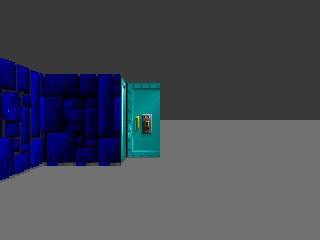
\includegraphics[scale=1.3]{screenshots/wolf3d_5_partialwalls_160rays.png}
 \caption{Finalez frame} \label{fig:mips}
 \end{figure}
 
 
 \begin{figure}[H]
\centering
 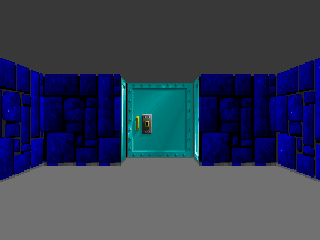
\includegraphics[scale=1.3]{screenshots/wolf4d_2_walls.png}
 \caption{3D Rendere Phase 2: Walls completed} \label{fig:mips}
 \end{figure}
 
 
 \begin{figure}[H]
\centering
 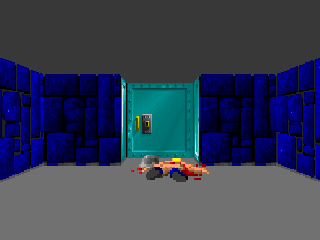
\includegraphics[scale=1.3]{screenshots/wolf3d_6_scaled}
 \caption{3D Rendere Phase 3: Scaled} \label{fig:mips}
 \end{figure}

 \begin{figure}[H]
\centering
 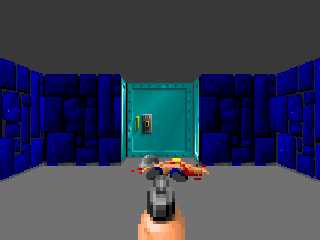
\includegraphics[scale=1.3]{screenshots/wolf3d_7_fullframe.png}
 \caption{3D Rendere Phase 2: Weapon} \label{fig:mips}
 \end{figure}
 

   Synergy: VGA column drawing, raycasting, occlusion array
   
\section{Fixed Point}

 
If integers were not accurate enough and floating points were too slow, how could trigonometry be done on those machines? The solution was to re-purpose the hardware via Fixed Points!\\
Fixed Point is a method that allows to keep track of fractions while still using the integer operations of the CPU. The machine manipulates what are supposed to be integer numbers but the programmers sees them as a real numbers. As usual it is easier to describe with a drawing. Integer are encoded following figure \ref{fig:int_layout}:
\begin{figure}[H]
\centering
 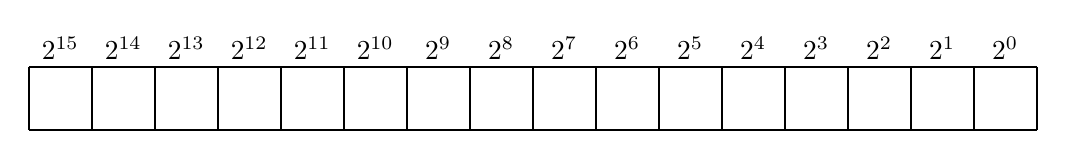
\begin{tikzpicture}[scale=0.8, every node/.style={scale=0.99}]
\draw[thick] (0,0) -- (16,0);
\draw[thick] (0,1) -- (16,1);
\foreach \i in {0,...,16}
{
     \draw[thick] (\i,1) -- (\i,0);
}

\foreach \i in {0,...,15}
{
     \node[] at (15-\i+0.5,1.3){$2^{\i}$}  ;
       
       
     
}
\end{tikzpicture}

 \caption{Integer layout.} \label{fig:int_layout}
 \end{figure}

So the value of the sequence of bits \emph{0010010010010010}:
\begin{figure}[H]
\centering
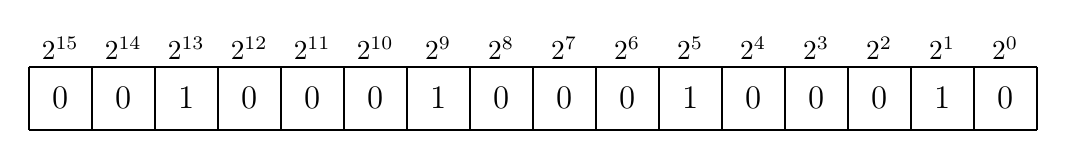
\begin{tikzpicture}[scale=0.8, every node/.style={scale=0.99}]
\draw[thick] (0,0) -- (16,0);
\draw[thick] (0,1) -- (16,1);
\foreach \i in {0,...,16}
{
     \draw[thick] (\i,1) -- (\i,0);
}

\foreach \i in {0,...,15}
{
     \node[] at (15-\i+0.5,1.3){$2^{\i}$}  ;
}

\tikzstyle{fontbf} = [font=\large]
\node[fontbf] at (0.5,0.5){0} ;
\node[fontbf] at (1.5,0.5){0};  
\node[fontbf] at (2.5,0.5){1} ; 
\node[fontbf] at (3.5,0.5){0} ;

\node[fontbf] at (4.5,0.5){0} ;
\node[fontbf] at (5.5,0.5){0};  
\node[fontbf] at (6.5,0.5){1} ; 
\node[fontbf] at (7.5,0.5){0} ;

\node[fontbf] at (8.5,0.5){0} ;
\node[fontbf] at (9.5,0.5){0};  
\node[fontbf] at (10.5,0.5){1} ; 
\node[fontbf] at (11.5,0.5){0} ;

\node[fontbf] at (12.5,0.5){0} ;
\node[fontbf] at (13.5,0.5){0};  
\node[fontbf] at (14.5,0.5){1} ; 
\node[fontbf] at (15.5,0.5){0} ;


\end{tikzpicture}

 \caption{Integer example.} \label{fig:mips}
 \end{figure}

 Is equal to $ 2^{13} + 2^9 + 2^5 + 2^1 =  8738 $.

\bigskip


Fixed Point arithmetic works by simply shifting the layout 8 bits to the left:
\begin{figure}[H]
 \centering
  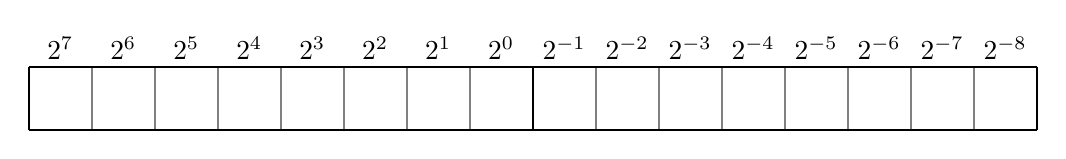
\begin{tikzpicture}[scale=0.8, every node/.style={scale=0.99}]


\colorlet{LighterMark}{black!50}

\foreach \i in {1,...,15}
{
     \draw[thick,LighterMark] (\i,1) -- (\i,0);
}

     \draw[thick,black] (0,1) -- (0,0);
      \draw[thick,black] (8,1) -- (8,0);
      \draw[thick,black] (16,1) -- (16,0);
      
\draw[thick,black] (0,0) -- (16,0);
\draw[thick,black] (0,1) -- (16,1);
 

%\foreach \i[evaluate={\pow=int(7-\i)}] in {0,...,7}
\foreach \i[evaluate={\pow=int(7-\i)}] in {0,...,7}
{
   \node[] at (\i+0.5,1.3){$2^{\pow}$  }  ;
      
         
     
}

%\foreach \i[evaluate={\pow=int((\i-7)*2)}]  in {8,...,15}
\foreach \i[evaluate={\pow=int(\i-7)}]  in {8,...,15}
{
     \node[] at (\i+0.5,1.3){$2^{-\pow}$}  ;
}




\end{tikzpicture}

 \caption{Fixed point layout.} \label{fig:mips}
\end{figure}

So the same sequence of bits \emph{0010010010010010}:
\begin{figure}[H]
 \centering
   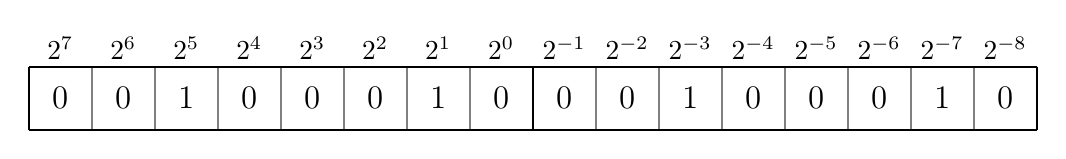
\begin{tikzpicture}[scale=0.8, every node/.style={scale=0.99}]


\colorlet{LighterMark}{black!50}

\foreach \i in {1,...,15}
{
     \draw[thick,LighterMark] (\i,1) -- (\i,0);
}

     \draw[thick,black] (0,1) -- (0,0);
      \draw[thick,black] (8,1) -- (8,0);
      \draw[thick,black] (16,1) -- (16,0);
      
\draw[thick,black] (0,0) -- (16,0);
\draw[thick,black] (0,1) -- (16,1);
 

%\foreach \i[evaluate={\pow=int(7-\i)}] in {0,...,7}
\foreach \i[evaluate={\pow=int(7-\i)}] in {0,...,7}
{
   \node[] at (\i+0.5,1.3){$2^{\pow}$  }  ;
      
         
     
}

%\foreach \i[evaluate={\pow=int((\i-7)*2)}]  in {8,...,15}
\foreach \i[evaluate={\pow=int(\i-7)}]  in {8,...,15}
{
     \node[] at (\i+0.5,1.3){$2^{-\pow}$}  ;
}

\tikzstyle{fontbf} = [font=\large]
\node[fontbf] at (0.5,0.5){0} ;
\node[fontbf] at (1.5,0.5){0};  
\node[fontbf] at (2.5,0.5){1} ; 
\node[fontbf] at (3.5,0.5){0} ;

\node[fontbf] at (4.5,0.5){0} ;
\node[fontbf] at (5.5,0.5){0};  
\node[fontbf] at (6.5,0.5){1} ; 
\node[fontbf] at (7.5,0.5){0} ;

\node[fontbf] at (8.5,0.5){0} ;
\node[fontbf] at (9.5,0.5){0};  
\node[fontbf] at (10.5,0.5){1} ; 
\node[fontbf] at (11.5,0.5){0} ;

\node[fontbf] at (12.5,0.5){0} ;
\node[fontbf] at (13.5,0.5){0};  
\node[fontbf] at (14.5,0.5){1} ; 
\node[fontbf] at (15.5,0.5){0} ;


\end{tikzpicture}

  \caption{Fixed point example.} \label{fig:mips}
\end{figure} 

Now represents:\\
\\
$ 2^5 + 2^1 = 34 $ for the integer part.\\
$ 2^{-3}+2^{-7} = 0.1328125 $ for the fractional part.\\
$ = 34.1328125$\\

\bigskip

The beauty of this method is that addition and subtraction work exactly like integers from the CPU instruction side:
  \bigskip
  DRAWING
  \bigskip


 The only special case is when performing operation.

\bigskip
  DRAWING
  \bigskip



 \textbf{\underline{Trivia :}}  Fixed Point Arithmetic usage was not limited to PC gaming. Many game console manufactured in the 90s and later had no hardware floating point unit: Sony's original PlayStation (1994) and Sega's Saturn (1994) are few examples among many with a design choice that not only reduced the production cost but also maximized the CPU pipeline throughput.
 
 
 
\begin{fancyquotes}
Much was made about the "ray casting" used in Wolfenstein, but the real reason for it was that I had a lot of trouble with wall-span rendering in Catacombs 3D.  C3D (and Hovertank before that) shipped with various graphics glitches that you could get in some combinations of map block configurations, position, and viewing angle.  Some were due to fixed point precision issues not being handled optimally, and some were due to clipping and culling issues that I didn’t really get a handle on until a couple years later.  In any case, they bothered me a lot.  Spurious graphics glitches do a lot of harm to the sense of immersion in a game, and I very much wanted Id games to feel “rock solid”.
 \bigskip \\
There was a clear performance cost to it – doing 320 traces through a tile map and treating each column independently is much slower than looping through a few long wall segments.  However, the resulting code was small and very regular compared to the hairball of my wall span renderers, and it did deliver the rock-solid feel I wanted.
 \bigskip \\
If you made extremely jagged block maps that would turn into many dozen independent wall segments, the ray casting could start to look like a good performance choice, but few scenes were even close to that.  This is exactly the same ray tracing versus rasterization performance tradeoff that is still being made today, but now it is “how many tens of millions of triangles per frame to ray tracing break-even” instead of “how many dozen wall segments”.
 \bigskip \\
\textbf{John Carmack - Programmer}
 \end{fancyquotes}
 

\end{document}

